\section{Appendices}
\subsection{Plots for the \code{paren} machine}
\label{plots_paren}
\begin{center}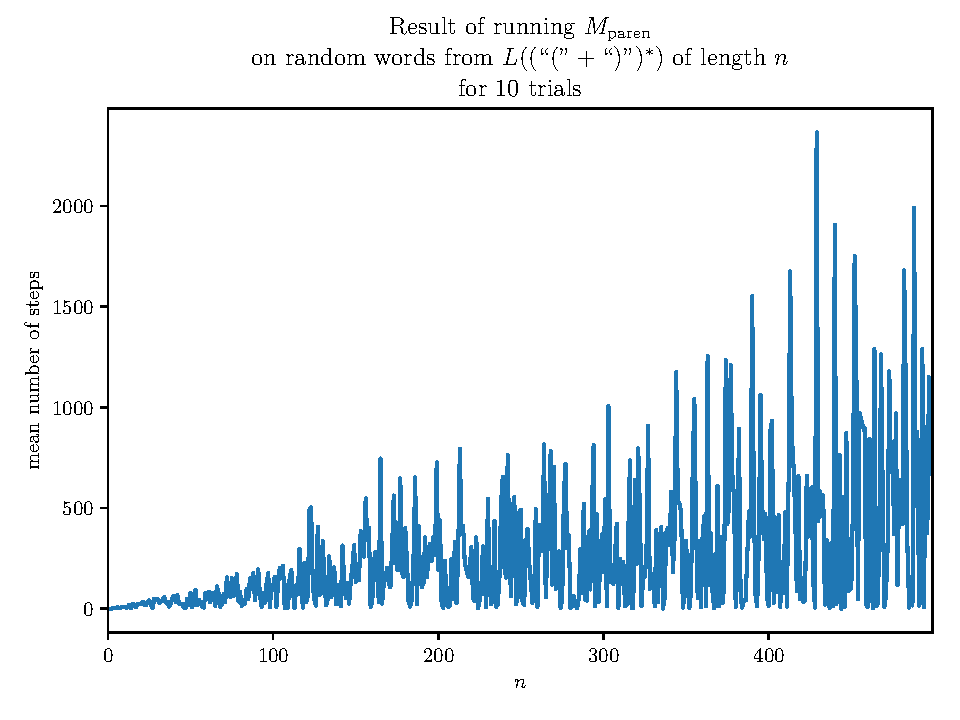
\includegraphics[width=\textwidth]{plots/paren-completely_random.pdf}\end{center}
\begin{center}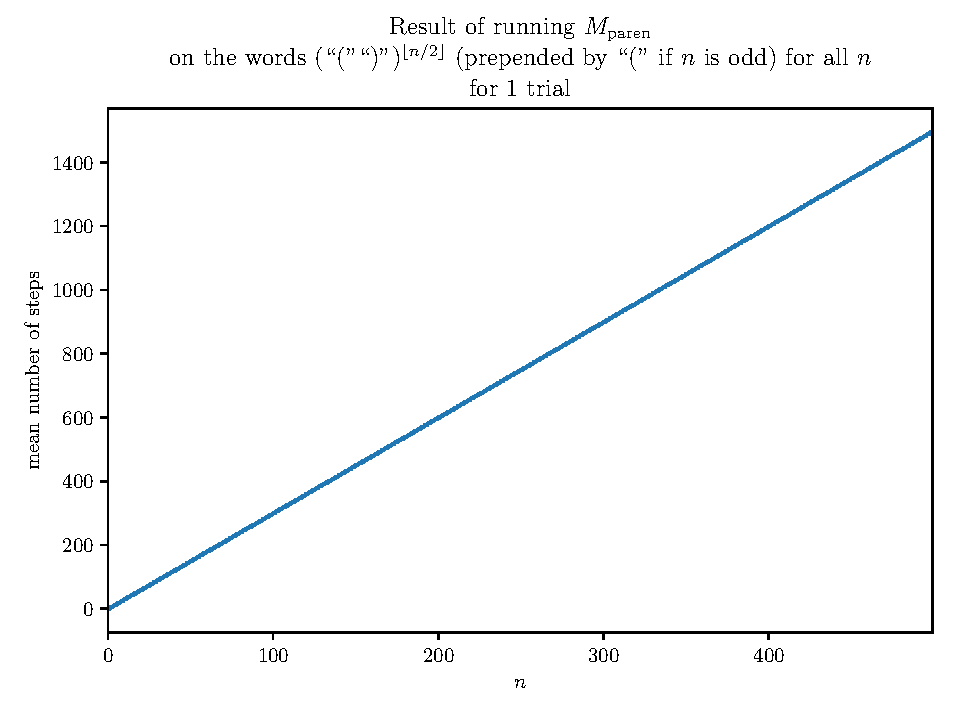
\includegraphics[width=\textwidth]{plots/paren-pairs.pdf}\end{center}
\begin{center}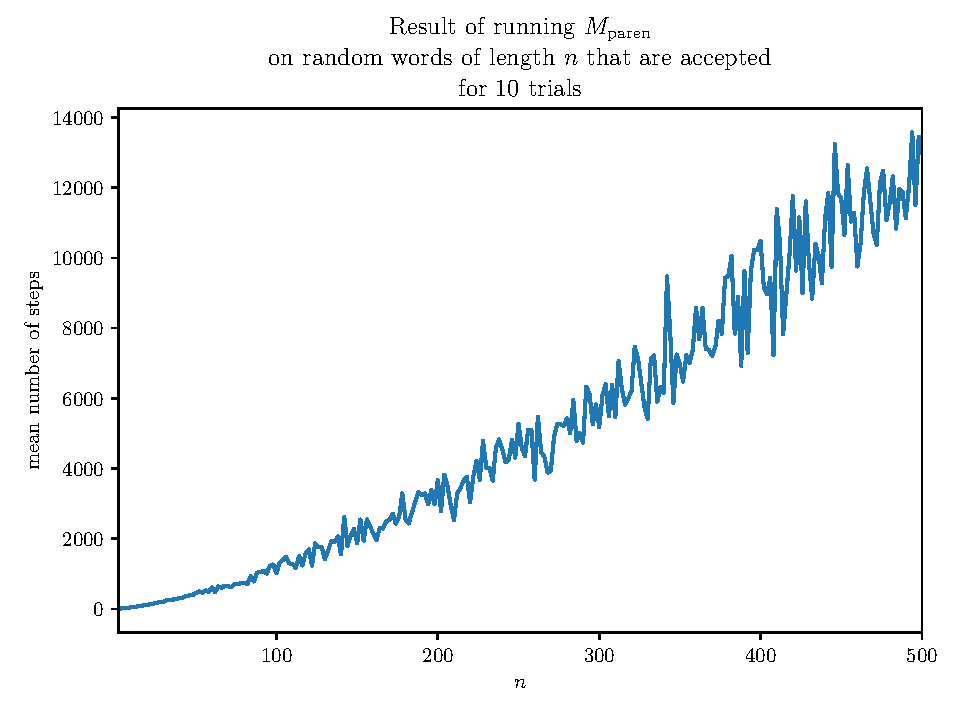
\includegraphics[width=\textwidth]{plots/paren-accepting_random.pdf}\end{center}
\begin{center}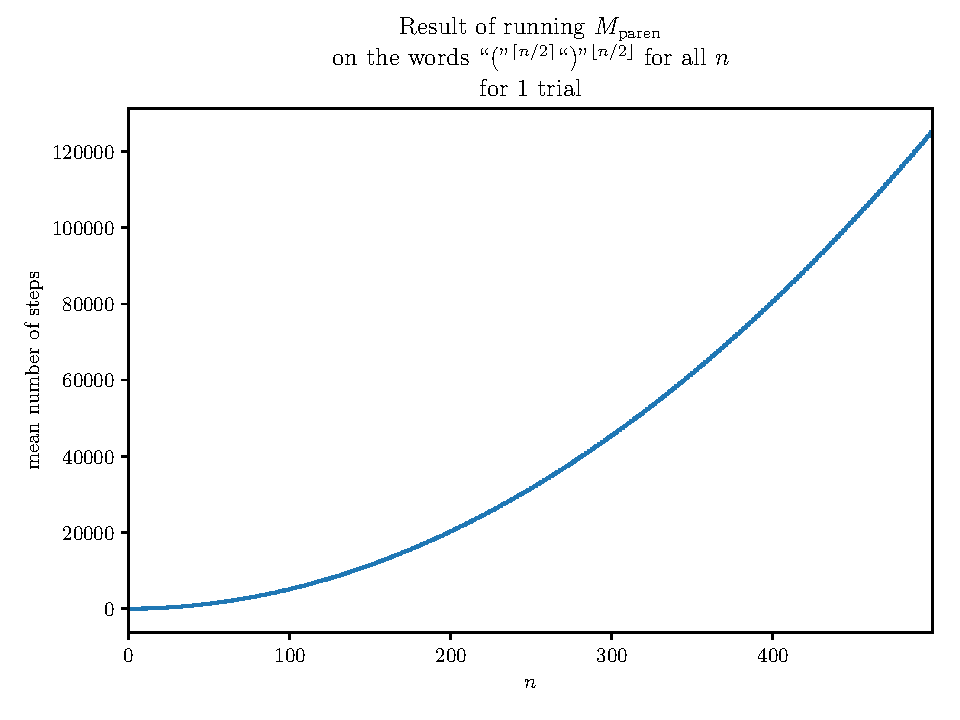
\includegraphics[width=\textwidth]{plots/paren-nested.pdf}\end{center}
\subsection{Plots for the \code{binadd} machine}
\label{plots_binadd}
\begin{center}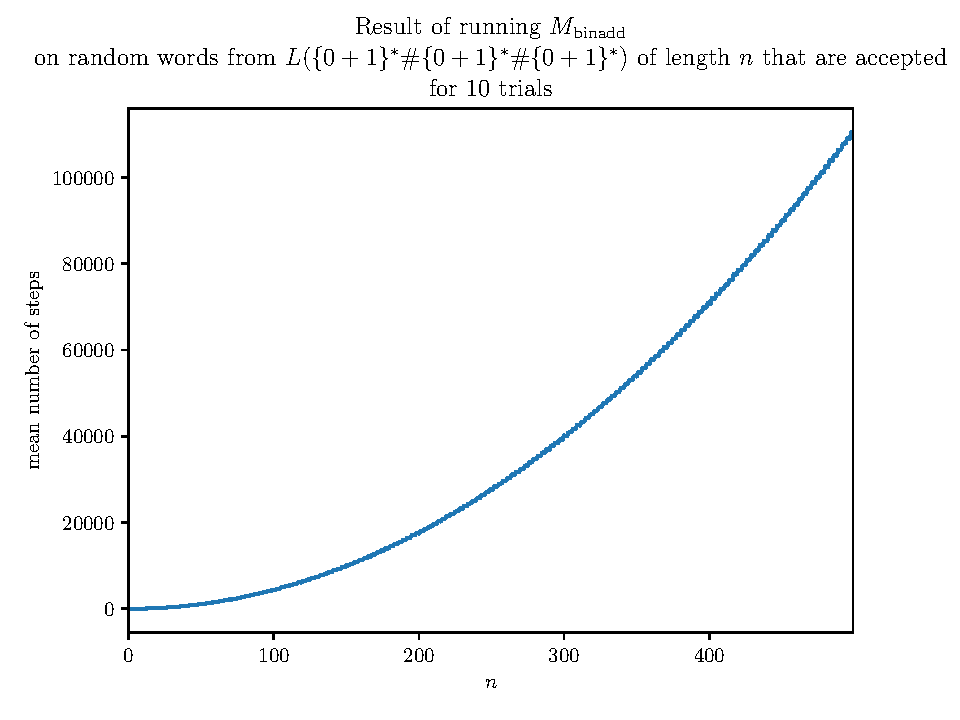
\includegraphics[width=\textwidth]{plots/binadd-accepting_random.pdf}\end{center}
\begin{center}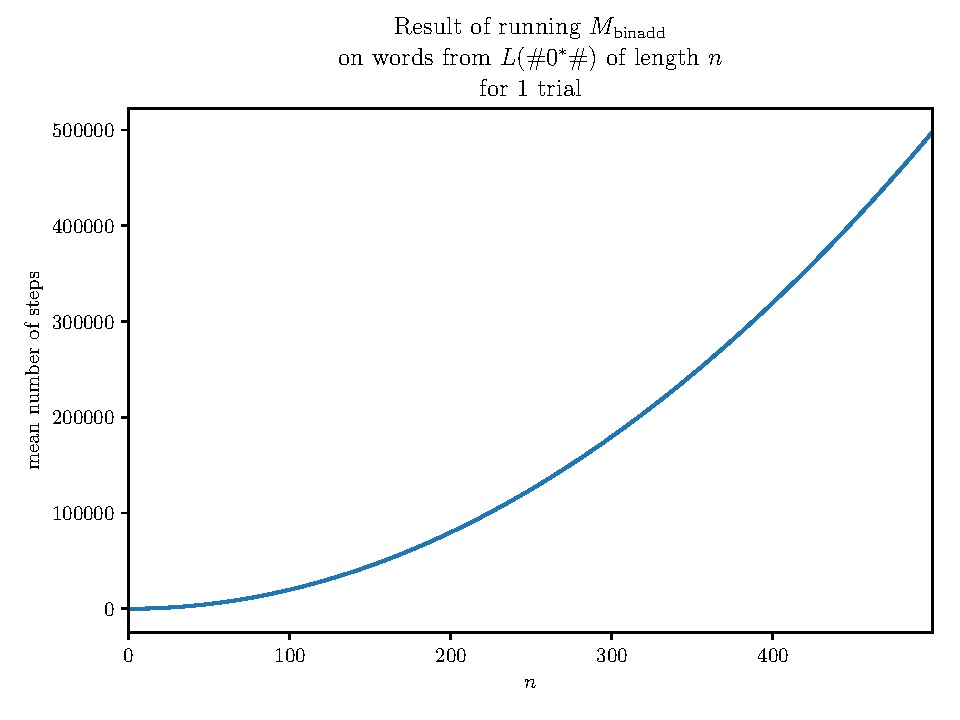
\includegraphics[width=\textwidth]{plots/binadd-accepting_zeros.pdf}\end{center}
\begin{center}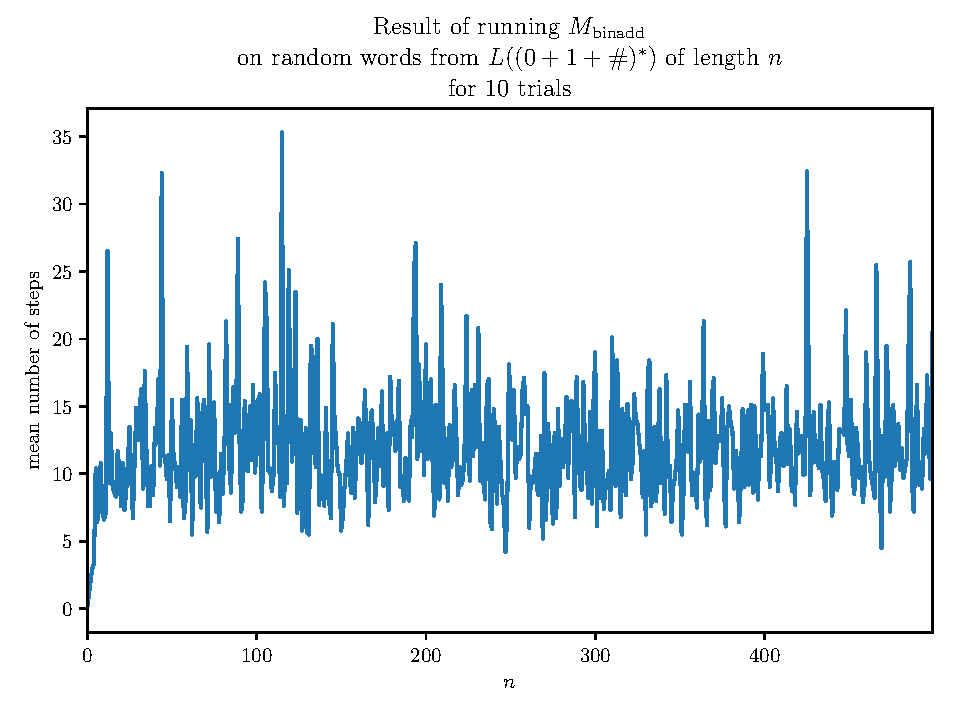
\includegraphics[width=\textwidth]{plots/binadd-completely_random.pdf}\end{center}
\begin{center}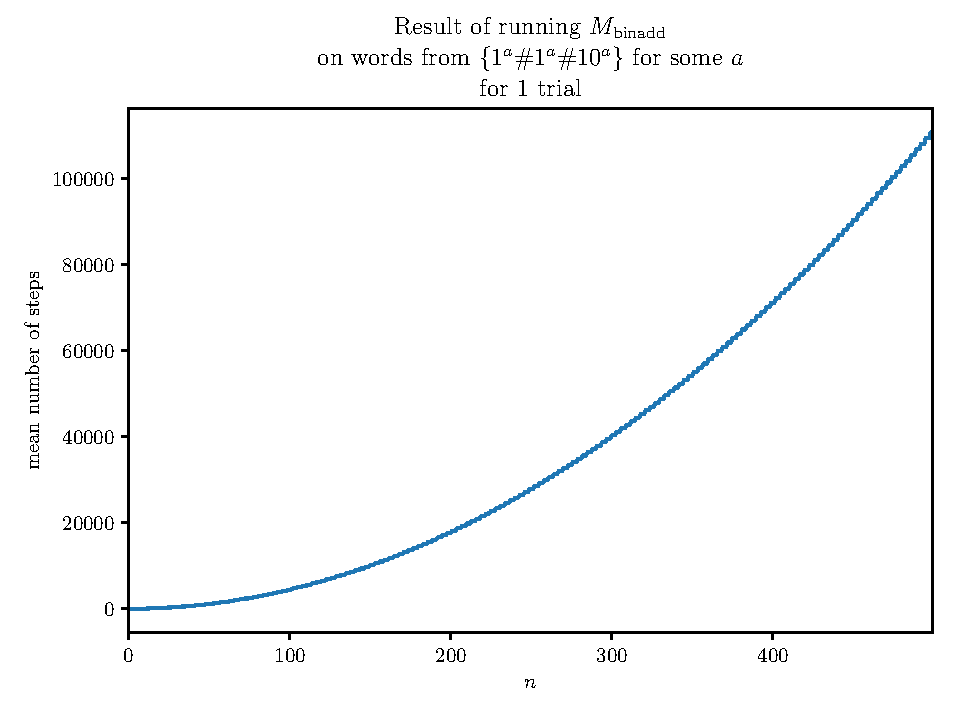
\includegraphics[width=\textwidth]{plots/binadd-accepting_ones.pdf}\end{center}
\begin{center}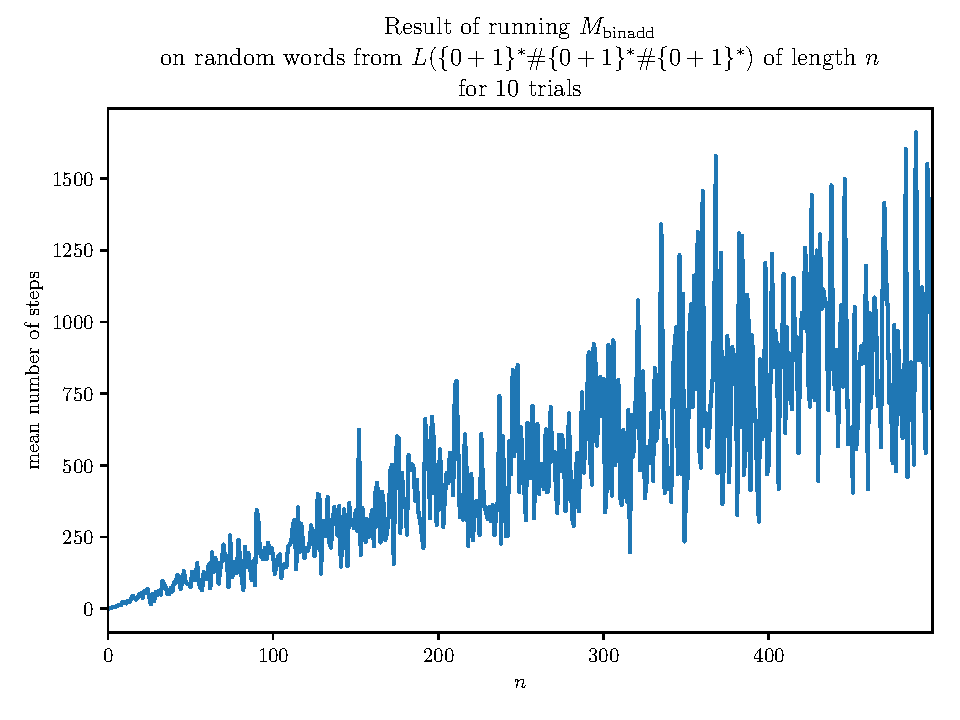
\includegraphics[width=\textwidth]{plots/binadd-random_three_numbers.pdf}\end{center}
\subsection{Plots for the \code{binaryunary} machine}
\label{plots_binaryunary}
\begin{center}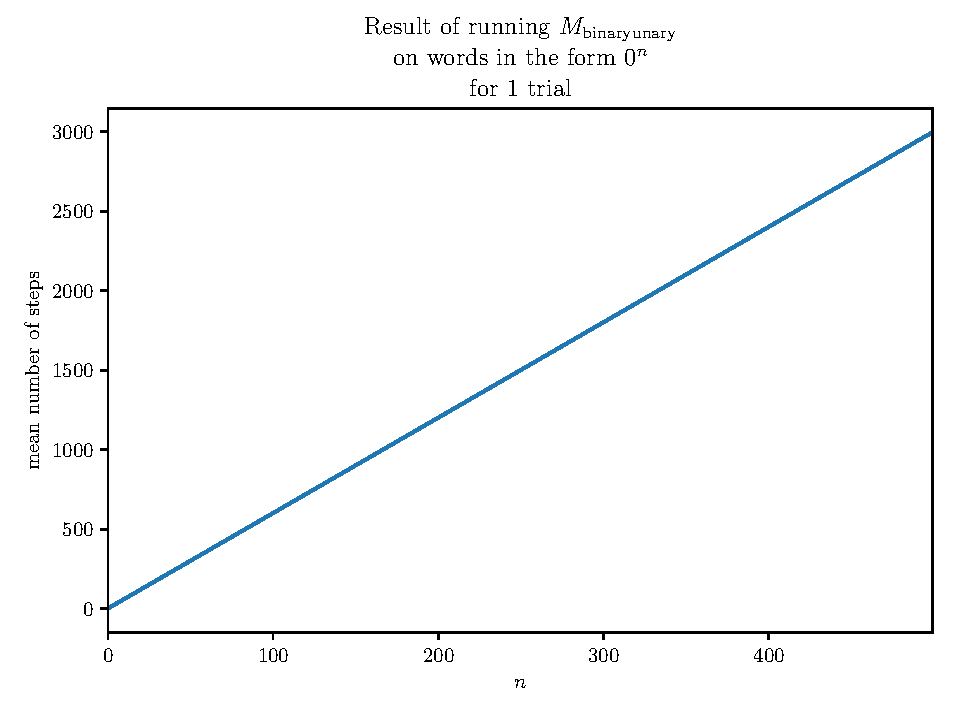
\includegraphics[width=\textwidth]{plots/binaryunary-zeros.pdf}\end{center}
\begin{center}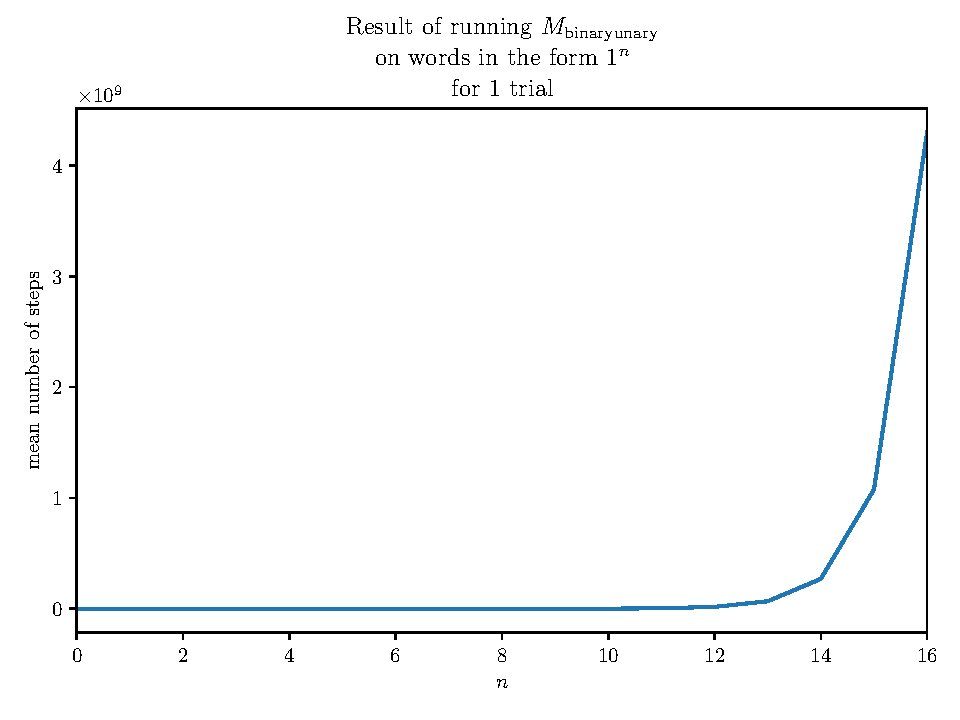
\includegraphics[width=\textwidth]{plots/binaryunary-ones.pdf}\end{center}
\subsection{Plots for the \code{subword} machine}
\label{plots_subword}
\subsection{Plots for the \code{subword\_fast} machine}
\label{plots_subword_fast}
